%% This is file `elsarticle-template-1-num.tex',
%%
%% Copyright 2009 Elsevier Ltd
%%
%% This file is part of the 'Elsarticle Bundle'.
%% ---------------------------------------------
%%
%% It may be distributed under the conditions of the LaTeX Project Public
%% License, either version 1.2 of this license or (at your option) any
%% later version.  The latest version of this license is in
%%    http://www.latex-project.org/lppl.txt
%% and version 1.2 or later is part of all distributions of LaTeX
%% version 1999/12/01 or later.
%%
%% The list of all files belonging to the 'Elsarticle Bundle' is
%% given in the file `manifest.txt'.
%%
%% Template article for Elsevier's document class `elsarticle'
%% with numbered style bibliographic references
%%
%% $Id: elsarticle-template-1-num.tex 149 2009-10-08 05:01:15Z rishi $
%% $URL: http://lenova.river-valley.com/svn/elsbst/trunk/elsarticle-template-1-num.tex $
%%
\documentclass[preprint,12pt]{elsarticle}

%% Use the option review to obtain double line spacing
%% \documentclass[preprint,review,12pt]{elsarticle}

%% Use the options 1p,twocolumn; 3p; 3p,twocolumn; 5p; or 5p,twocolumn
%% for a journal layout:
%% \documentclass[final,1p,times]{elsarticle}
%% \documentclass[final,1p,times,twocolumn]{elsarticle}
%% \documentclass[final,3p,times]{elsarticle}
%% \documentclass[final,3p,times,twocolumn]{elsarticle}
%% \documentclass[final,5p,times]{elsarticle}
%% \documentclass[final,5p,times,twocolumn]{elsarticle}

%% if you use PostScript figures in your article
%% use the graphics package for simple commands
%% \usepackage{graphics}
%% or use the graphicx package for more complicated commands
%% \usepackage{graphicx}
%% or use the epsfig package if you prefer to use the old commands
%% \usepackage{epsfig}

%% The amssymb package provides various useful mathematical symbols
\usepackage{amssymb}
%% The amsthm package provides extended theorem environments
%% \usepackage{amsthm}

%% The lineno packages adds line numbers. Start line numbering with
%% \begin{linenumbers}, end it with \end{linenumbers}. Or switch it on
%% for the whole article with \linenumbers after \end{frontmatter}.
\usepackage{lineno}
\usepackage{hyperref}

%% natbib.sty is loaded by default. However, natbib options can be
%% provided with \biboptions{...} command. Following options are
%% valid:

%%   round  -  round parentheses are used (default)
%%   square -  square brackets are used   [option]
%%   curly  -  curly braces are used      {option}
%%   angle  -  angle brackets are used    <option>
%%   semicolon  -  multiple citations separated by semi-colon
%%   colon  - same as semicolon, an earlier confusion
%%   comma  -  separated by comma
%%   numbers-  selects numerical citations
%%   super  -  numerical citations as superscripts
%%   sort   -  sorts multiple citations according to order in ref. list
%%   sort&compress   -  like sort, but also compresses numerical citations
%%   compress - compresses without sorting
%%
%% \biboptions{comma,round}

% \biboptions{}


\journal{GSoC KDE 2017}

\begin{document}

\begin{frontmatter}

%% Title, authors and addresses

%% use the tnoteref command within \title for footnotes;
%% use the tnotetext command for the associated footnote;
%% use the fnref command within \author or \address for footnotes;
%% use the fntext command for the associated footnote;
%% use the corref command within \author for corresponding author footnotes;
%% use the cortext command for the associated footnote;
%% use the ead command for the email address,
%% and the form \ead[url] for the home page:
%%
%% \title{Title\tnoteref{label1}}
%% \tnotetext[label1]{}
%% \author{Name\corref{cor1}\fnref{label2}}
%% \ead{email address}
%% \ead[url]{home page}
%% \fntext[label2]{}
%% \cortext[cor1]{}
%% \address{Address\fnref{label3}}
%% \fntext[label3]{}

\title{Porting activities in GCompris in Qt-Quick}

%% use optional labels to link authors explicitly to addresses:
%% \author[label1,label2]{<author name>}
%% \address[label1]{<address>}
%% \address[label2]{<address>}

\author{Rudra Nil Basu}

\address{ \textbf{Email ID}: rudra.nil.basu.1996@gmail.com}
\address{ \textbf{Freenode IRC Nick}: rudra}
\address{ \textbf{Location}: Kolkata, West Bengal, India UTC+5.30}
%\address{ \textbf{Mentor}: Bruno Coudoin (bruno.coudoin@gcompris.net)}
%\address{ \textbf{Co-Mentor}: Johnny Jazeix (jazeix@gmail.com), }

\end{frontmatter}

%%
%% Start line numbering here if you want
%%
%\linenumbers

%% main text
\section{Motivation}
\label{S:1}

%GCompris is about teaching the basics in the most easiest way to children between the age of 2 to 10. The gtk+ version of GCompris was very well recieved, and from there it was decided to Qt version, to make GCompris available for all kinds of devices, like tablets. The latest version of GCompris is 0.70 and as of now it has 137 categories on various topics like science, maths, games and much more, fully supporting 15 languages.

GCompris is a high quality educational suite which aims at making learning easier for children aged 2 to 10. GCompris currently has 137 activities on various topics such as science, maths, games with which it has succesfully created a great learning environment for children. I strongly believe in what GCompris stands for and in this project I aim at taking GCompris one step forward by finishing three started activities: \textit{Pilot a Submarine} , \textit{Garbage Recycle} and \textit{Object Arrangement}


%As of \today , a brief statistics of GCompris are:
%\begin{itemize}
%\item Latest Version: 0.70
%\item A total of 137 categories on various topics like science, maths, games and much more.
%\item 15 languages fully supported
%\item More than 100000 downloads on the Google Play Store
%\item The new version contains 8 new activities
%\end{itemize}

%My goal for the project is to port two experimental activities from the Gtk+ version of GCompris to the Qt version.

%The best way to teach any concept is by demonstration. But it is not always possible to demonstrate everything that needs to be taught, such as the working of submarine and it's different parts. That's were simulation of real world problems come to play. The aim of this project is to simulate real world situations in two activities, \textit{"Pilot a Submarine"} and \textit{"Sea race (Single Player)"}

\section{Project Goals}
\label{S:1}

By the end of the Google Summer of Code's time period, I will be completing the following activities :

\begin{itemize}

\item \textbf{Pilot a Submarine}: It is a port to the Qt version of a strategic activity originally present in the Gtk+ version aimed to teach how a submarine works. It was started in this branch: 

\href{https://cgit.kde.org/gcompris.git/log/?h=gsoc-submarine}{https://cgit.kde.org/gcompris.git/log/?h=gsoc-submarine}

\item \textbf{Garbage Recycle}: This activity is aimed to teach garbage classification. This was started in \href{https://cgit.kde.org/gcompris.git/log/?h=SoK_Activity_recyclebin_shivansh} {recyclebin} branch

Discussions:

\href{https://phabricator.kde.org/T339}{https://phabricator.kde.org/T339}

%\item \textbf{The Solar System}: This activity aims at providing a basic understanding about our Solar System, it's planets and facts and properties of each of the planets.

\item \textbf{Object Arrangement}: This activity is aimed at teaching arranging objects in a given order based on factors like height and width.

The activities for arranging numbers and alphabets in either ascending or descending order is already in progress and this will be a generic one, adding all kinds of ordering activities to the project.

Discussions:

\href{https://phabricator.kde.org/T1956}{https://phabricator.kde.org/T1956}
\end{itemize}

\section{Implementation Details}
\label{S:1}

\subsection{Pilot a Submarine}

The  \textit{"Pilot a Submarine"} is to learn how a submarine works, explaining the usage of elements such as engine, rudders and air tanks, in order to navigate a submarine to a required depth.

\begin{itemize}


\item Since this activity was already present in the Gtk+ version, I will be using the svg and the audio files from the resources used in the Gtk+ submarines activity. This will allow me to dive into the coding part directly. 

\item There will be a tutorial at the start of the activity, which will give a brief description about the different elements (engine, rudders and air tanks) and it's functions.

\item Firstly I will be implementing the submarine and the mechanics of it's elements, namely the engine, rudders and the air tanks. Once that is in place, I will then shift on to create various levels and it's variations.

%The Gtk+ version had only 4 levels, and I will increase the number of levels in the Qt port, increasing the difficulty curve, bringing up elements like caves, rocks, while still keeping it doable for children within the prescribed age limit.

\item The activity will contain pickups in the form of jewels, as it was present in the Gtk+ version

\item Besides the regular pickups in the Gtk+ version, there will be additional threats in the form of rocks and caves, in order to maintain an increasing difficulty curve, while still keeping it doable for children within the prescribed age limit.

\item In order to enhance the experience, the overall activity and the movement of the submarine and the animations will be smoother compared to the Gtk+ activity.

\begin{figure}[h]
\centering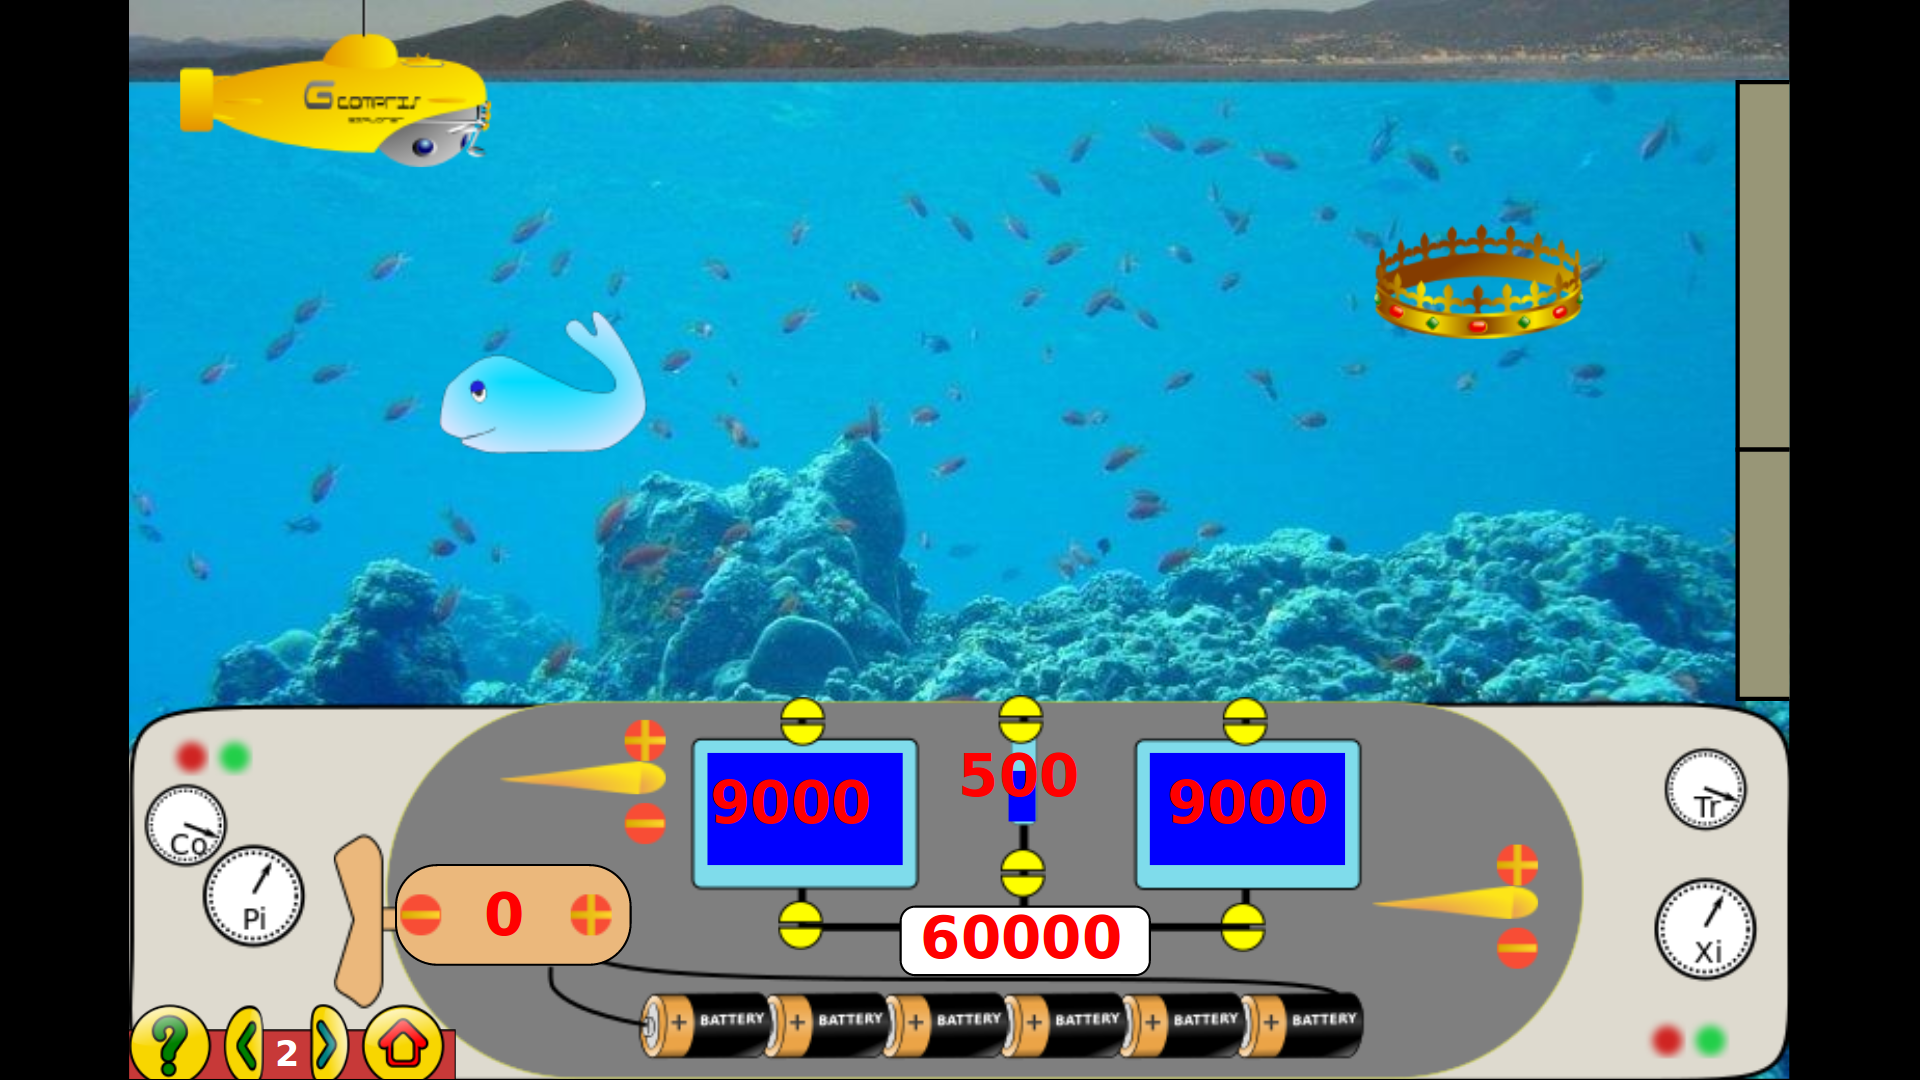
\includegraphics[width=1.0\linewidth]{submarine}
\caption{Submarine Activity}
\end{figure}

\end{itemize}
\subsection{Garbage Recycle}

This activity will be done from scratch as the implementation in the given branch doesn't match with the description. I will be using images from \href{https://openclipart.org/}{openclipart.org} and it will have the following features:

\begin{itemize}

\item The activity will begin with a tutorial explaining the basics of different types of recycling procedure for different materials, along with the goal of the activity.

\item Garbages of different types will be available in the table at the start of each level.

\item The user will have to put the waste materials in it's correct recycling bin. On placing the waste in it's correct bin, it will be recycled properly. The goal of the activity is to correctly recycle each of the wastes as provided in each levels.

\item Items will be placed on it's respective bin via drag and drop

\item With progress of levels, there will be an increase in the categories of waste materials, in order to maintain a proper difficulty curve.

\end{itemize}

\subsection{Object Arrangement}

This activity will be created from scratch, in order to expand the current ordering activity to a more generic version of it. It will have the following features:

\begin{itemize}

\item Different types of objects will be provided at the start of each levels and the user will be asked to arrange them in a specific order (ascending or descending) based on a given parameter (height or weight)

\item A toolbox will be provided to the user with the help of which the user can measure the required property of an item

\item The measured properties will be marked on the object. If a property of an object is not yet measured, it will be marked as unknown.

\item With the proper measurements, the user will then arrange the items in the correct order of the parameter

\end{itemize}

%/*2d matrix, Tux, door and few pickups. command tux to take all pickups and move out of the door. Commands - rotate (+-90, +180), move forward (x blocks)*/

%/*Physics*/

%/*Complete incomplete activities*/

% Garbage, ordering, Solar system, family

\section{Timeline}
\label{S:1}

\section{About Me}
\label{S:1}

I am a third year undergraduate engineering student from West Bengal University of Technology, pursuing B.Tech in Computer Science and Engineering. I have been contributing to KDE for the past few months on the Qt version of GCompris.

My contributions on GCompris include:

\begin{itemize}

\item Display the characters attempted by the user in the Hangman activity

\href{https://github.com/gcompris/GCompris-qt/commit/8ab75acf49431c685021f3cd0e58cf31f3fa4568}{https://github.com/gcompris/GCompris-qt/commit/\\8ab75acf49431c685021f3cd0e58cf31f3fa4568}

\item Adding a Directory class in Core to directly get a list of all files in a given directory

\href{https://github.com/gcompris/GCompris-qt/commit/955462b943c34fc130d1a68fcfb0e1ec6393a3f0}{https://github.com/gcompris/GCompris-qt/commit/\\955462b943c34fc130d1a68fcfb0e1ec6393a3f0}

\item Improve the algorithm to add new levels in the categorization activity, so that we do not need to change the code while adding new levels. Also, added odd-even category in the categorization activity

\href{https://github.com/gcompris/GCompris-qt/commit/db7a4a9b743a3521c7c68f0b2b54719cbc9582db}{https://github.com/gcompris/GCompris-qt/commit/\\db7a4a9b743a3521c7c68f0b2b54719cbc9582db}

\item Display a black point in drawletters and drawnumbers activity whenever a line cannot be drawn for a given input

\href{https://github.com/gcompris/GCompris-qt/commit/eaf8dd326dd3f5581995155739be5c72af744f92}{https://github.com/gcompris/GCompris-qt/commit/\\eaf8dd326dd3f5581995155739be5c72af744f92}

\item \textbf{Ongoing activity}: Ordering activity, which aims at arranging numbers and alphabets in it's increasing or decreasing order

\href{https://github.com/gcompris/GCompris-qt/pull/172}{https://github.com/gcompris/GCompris-qt/pull/172}

\end{itemize}

Besides this, I am the head of our college's programming club, where we create awareness about open source and encourage newcomers to take part in open source contribution.

\textbf{Blog}: \href{http://rudranilbasu.me/blog/}{rudranilbasu.me/blog}

%% The Appendices part is started with the command \appendix;
%% appendix sections are then done as normal sections
%% \appendix

%% \section{}
%% \label{}

%% References
%%
%% Following citation commands can be used in the body text:
%% Usage of \cite is as follows:
%%   \cite{key}          ==>>  [#]
%%   \cite[chap. 2]{key} ==>>  [#, chap. 2]
%%   \citet{key}         ==>>  Author [#]

%% References with bibTeX database:

\bibliographystyle{model1-num-names}
\bibliography{sample.bib}

%% Authors are advised to submit their bibtex database files. They are
%% requested to list a bibtex style file in the manuscript if they do
%% not want to use model1-num-names.bst.

%% References without bibTeX database:

% \begin{thebibliography}{00}

%% \bibitem must have the following form:
%%   \bibitem{key}...
%%

% \bibitem{}

% \end{thebibliography}


\end{document}

%%
%% End of file `elsarticle-template-1-num.tex'.
